\documentclass[linenumbers,floatfix,ApJL,twocolumn]{aastex631}

% \pdfoutput=1

% %\usepackage{lmodern}
\usepackage{microtype}
% \usepackage{url}
% \usepackage{amsmath}
% \usepackage{amssymb}
% \usepackage{natbib}
% \usepackage{multirow}
% \usepackage{graphicx}
% \bibliographystyle{aasjournal}

% \usepackage{mathtools}
% \usepackage{calc}
% \usepackage{etoolbox}
% \usepackage{xspace}
% \usepackage[T1]{fontenc} % https://tex.stackexchange.com/a/166791
% \usepackage{textcomp}
\usepackage{ifxetex}
\ifxetex
\usepackage{fontspec}
\defaultfontfeatures{Extension = .otf}
\fi
\usepackage{fontawesome}


% references to text content
\newcommand{\documentname}{\textsl{Article}}
\newcommand{\figureref}[1]{\ref{fig:#1}}
\newcommand{\Figure}[1]{Figure~\figureref{#1}}
\newcommand{\figurelabel}[1]{\label{fig:#1}}
\newcommand{\eqref}[1]{\ref{eq:#1}}
\newcommand{\Eq}[1]{Equation~(\eqref{#1})}
\newcommand{\eq}[1]{\Eq{#1}}
\newcommand{\eqalt}[1]{Equation~\eqref{#1}}
\newcommand{\eqlabel}[1]{\label{eq:#1}}

% TODOs
\newcommand{\todo}[3]{{\color{#2}\emph{#1}: #3}}
\newcommand{\dfmtodo}[1]{\todo{DFM}{red}{#1}}
\newcommand{\avi}[1]{\todo{Avi}{orange}{#1}}
\newcommand{\alltodo}[1]{\todo{TEAM}{red}{#1}}
\newcommand{\citeme}{{\color{red}(citation needed)}}


% % typography obsessions
% \setlength{\parindent}{3.0ex}

% % from: https://github.com/rodluger/corTeX
% % Add code, proof, and animation hyperlinks
% \definecolor{linkcolor}{rgb}{0.1216,0.4667,0.7059}
% \newcommand{\codeicon}{{\color{linkcolor}\faFileCodeO}}
% \newcommand{\prooficon}{{\color{linkcolor}\faPencilSquareO}}
% \input{gitlinks}

% % Define a proof environment for open source equation proofs
% \newtagform{eqtag}[]{(}{)}
% \newcommand{\currentlabel}{None}
% \newenvironment{proof}[1]{%
% \ifstrempty{#1}{%
% \renewtagform{eqtag}[]{\raisebox{-0.1em}{{\color{red}\faPencilSquareO}}\,(}{)}%
% }{%
% \renewtagform{eqtag}[]{\prooflink{#1}\,(}{)}%
% }%
% \usetagform{eqtag}%
% \renewcommand{\currentlabel}{#1}
% \align%
% }{%
% \endalign%
% \renewtagform{eqtag}[]{(}{)}%
% \usetagform{eqtag}%
% \message{<<<\currentlabel: \theequation>>>}%
% }

% % Define the `oscaption` command for open source figure captions
% \newcommand{\oscaption}[2]{\caption{#2 \codelink{#1}}}

% Projects:
\newcommand{\project}[1]{\textsf{#1}}

\newcommand{\python}{\project{Python}}
\newcommand{\cython}{\project{Cython}}
\newcommand{\cpp}{\project{C++}}
\newcommand{\jupyter}{\project{Jupyter}}

\newcommand{\exoplanet}{\project{exoplanet}}
\newcommand{\lightkurve}{\project{lightkurve}}
\newcommand{\starry}{\project{starry}}
\newcommand{\radvel}{\project{RadVel}}
\newcommand{\batman}{\project{batman}}
\newcommand{\theano}{\project{Theano}}
\newcommand{\pymc}{\project{PyMC3}}
\newcommand{\celerite}{\project{celerite}}
\newcommand{\isochrones}{\project{isochrones}}
\newcommand{\dynesty}{\project{dynesty}}
\newcommand{\astroquery}{\project{astroquery}}
\newcommand{\jupytetr}{\project{astroquery}}

\newcommand{\tess}{\project{TESS}}
\newcommand{\kepler}{\project{Kepler}}
\newcommand{\gaia}{\project{Gaia}}

\newcommand{\cks}{\project{CKS}}
\newcommand{\mesa}{\project{MESA}}
\newcommand{\mast}{\project{MAST}}
\newcommand{\mist}{\project{MIST}}
\newcommand{\exofop}{\project{ExoFOP}}

% math
\newcommand{\T}{\ensuremath{\mathrm{T}}}
\newcommand{\dd}{\ensuremath{ \mathrm{d}}}
\newcommand{\unit}[1]{{\ensuremath{ \mathrm{#1}}}}
\newcommand{\bvec}[1]{{\ensuremath{\boldsymbol{#1}}}}




\newif\ifdraft
\drafttrue % switch to false in non-draft version (thereby hiding the todos)
\newcommand{\inDraftVersion}[1]{\ifdraft #1\fi} 


% TODOs
\newcommand{\todo}[3]{\inDraftVersion{{\color{#2}\emph{#1}: #3}}}
\newcommand{\dfmtodo}[1]{\todo{DFM}{red}{#1}}
\newcommand{\avi}[1]{\todo{Avi}{red}{#1}}
\newcommand{\alltodo}[1]{\todo{TODO}{red}{#1}}
\newcommand{\citeme}{{\color{red}(citation needed)}}


\newcommand{\red}{\textcolor{red}}
\newcommand{\textuit}[1]{\textit{\underline{#1}}}



%% Numbers
% https://exoplanetarchive.ipac.caltech.edu/docs/counts_detail.html
% https://exoplanetarchive.ipac.caltech.edu/index.html

\newcommand{\numConfirmedPlanets}{5,090} % 
\newcommand{\numCandidatesRemaining}{6,959}

\newcommand{\numTessCandidates}{5,488} % 
\newcommand{\numTessPlanets}{227}
\newcommand{\numAnalysed}{2,833}
\newcommand{\numAnalysedMulti}{151}
\newcommand{\numAnalysedSingle}{68}
\newcommand{\cpuHrs}{$\sim80,000\ \rm{Hrs}$}

%% links

% % % from: https://github.com/rodluger/corTeX
% % % Add code, proof, and animation hyperlinks
% \definecolor{linkcolor}{rgb}{0.1216,0.4667,0.7059}
% \newcommand{\codeicon}{{\color{linkcolor}\faFileCodeO}}

% % % Define the `oscaption` command for open source figure captions
% \newcommand{\oscaption}[2]{\caption{#2 \codelink{#1}}}


% \makeatletter
\newcommand{\github}[1]{\href{#1}{\textcolor{gray}{\faGithubSquare}}}








\shorttitle{The \tess\ Atlas}
\shortauthors{the authors}

\begin{document}

\title{The \tess\ Atlas: an open source catalog of TESS transit fits}

% ADS bibliography link
% https://ui.adsabs.harvard.edu/user/libraries/_DyLS4HbTY-eJIMBiFUdxw

\author{Author list TBD}
% \correspondingauthor{Daniel Foreman-Mackey}
\email{foreman.mackey@gmail.com}

\author[0000-0002-4146-1132{Avi Vajpeyi}
\affiliation{
    School of Physics and Astronomy,
    Monash University,
    Clayton VIC 3800,
    Australia
}
\affiliation{
OzGrav: The ARC Centre of Excellence for Gravitational Wave Discovery,
Clayton VIC 3800,
Australia
}

\author[0000-0002-9328-5652]{Daniel Foreman-Mackey}
\affiliation{
    Center for Computational Astrophysics,
    Flatiron Institute,
    162 5th Ave,
    New York, NY 10010
}







\begin{abstract}
We present the first \tess\ Atlas, a transiting exoplanet parameter estimate catalog generated from 2-minute cadence \tess\ data during 2018 through 2022 (Sectors 1 to 54).
This contains posterior estimates for \red{\numAnalysed} \tess\ Objects of Interest, including \red{\numAnalysedMulti} multi-planet candidate systems and \red{\numAnalysedSingle} candidates with data for only a single transit. 
Our analysis utilises the No-U-Turns Markov chain Monte Carlo algorithm to sample the parameter space with a circular transit model implemented in \exoplanet. 
To enable follow-up as our understanding of the underlying populations evolves, we provide posterior samples from our analyses and Jupyter notebooks to reproduce the analyses for each exoplanet candidate.
\end{abstract}

% info on sectors: https://heasarc.gsfc.nasa.gov/docs/tess/sector.html

\keywords{%
  methods: data analysis ---
  methods: statistical ---
  miscellaneous --- catalogs --- surveys
}


\section{Introduction} \label{sec:intro}

In July 2020, NASA’s Transiting Exoplanet Survey Satellite \citep{Ricker:2015:JATIS} completed its two-year Primary Mission to search for transiting exoplanets around nearby bright stars. 
\tess\ recorded 2-minute cadence observations for $\sim200,000$ pre-selected stars that were processed by the \tess\ Science Processing Operations Center \citep{Jenkins:2016:SPIE} pipeline. 
Additionally, \tess\ also recorded measurements of its entire field of view in 10 and 30-minute sampled full-frame images (FFIs), enabling the flux measurements of tens of millions of stars. 
Between 2, 10 and 30-minute observations, the \tess\ Primary Mission and the ongoing extended missions have identified over \red{$\numTessCandidates$} planet candidates, \red{$\numTessPlanets$} of which have been confirmed as planets \citep{Stassun:2018:AJ, Stassun:2019:AJ, Guerrero:2021:ApJS, Guerrero:2021:AAS}. 
Furthermore, \tess\ data have provided numerous non-exoplanet candidates disclosing new information on eclipsing binaries (e.g., ), and tidally interacting systems (e.g., ), exomoons (e.g., ), comets (e.g., ),  exocoments (e.g., ), supernovae (e.g., ), and more (see [review] for more). \alltodo{get citations}.

In this work we provide a comprehensive catalog of transiting exoplanet posterior estimates for the \red{\numAnalysed} \tess\ Objects of Interest (TOIs) with 2-minute cadence observations from 2018 through 2022. 
The posterior distributions provide robust uncertainties for the circular transit model's planet orbital timing parameters, stellar limb darkening, stellar density, mean flux and detector-noise parameters. 
The posterior distributions can allow future researchers to study the planet population in detail and assess the reliability of the most Earth-like candidates, \alltodo{list more things that can be done}.

The remainder of the paper is organised as follows: Section~\ref{sec:method} describes our transit light curve model and the Bayesian framework we use to estimate parameters of exoplanet systems from the observed data. 
The analysis results are summarised in Section~\ref{sec:results}.
The catalog, released data, and software to reproduce the results are described in Section~\ref{sec:data} and are available online as supplementary materials (\atlasUrl).
Finally, we provide concluding remarks in Section~\ref{sec:conclusion}.

\section{Method} \label{sec:method}

\alltodo{TOI selection, lightcurve preprocessing, eccentricity posterior postprocessing}

\subsection{Transit light curve model}

There are many options for parameterisation of a transit, but we choose to model these transits as circular, non-interacting Keplerian orbits around their host star, parameterised by their observables. 
We approximate the host star's stellar limb darkening profile using \citet{Kipping:2013:MNRAS}'s quadratic limb darkening law.
Finally, we compute the exoplanet's resultant quadratic limb-darkened transit lightcurve using an analytical model implemented in \starry.
The stellar variables in this model are parameterised by
the baseline relative flux of the light curve $f_0$,
the mean stellar density $\rho_\star$,
and two parameters describing the quadratic limb-darkening profile of the
star $u_1, u_2$.
To model stellar variability (e.g. asteroseismic oscillation of the star)  we use a Gaussian Process implemented in \celerite\ with a stochastically driven damped harmonic oscillator kernel in linear combination with a jitter term, to capture misspecified error bars and model misspecification. This requires three parameters: the quality factor $Q_{\rm GP}$, the undamped period of the oscillator $\rho_{\rm GP}$, the standard deviation of the process $\sigma_{\rm GP}$.

Each of the $n$ exoplanets in the system are parameterised by the planets'
\begin{enumerate}
  \item \emph{two reference transit times}, one near the beginning of the observations, $t_{\rm min}[n]$, and one near the end, $t_{\rm max}[n]$, measured in \tess\ BJD,
  \item \emph{the approximate transit depth}, $\delta[n]$, measured in parts-per-thousand,
  \item \emph{the impact parameter} of the orbit, $b[n]$, constrained to be $|b| \le 1$, and
  \item \emph{the transit duration}, $\tau[n]$, measured in hours,
  \item \emph{the radius ratio} $k[n]$ of the planet radius $R_{\rm p}[n]$ divided by the stellar radius $R_\star$.
\end{enumerate}
In the case when there are a planet has only a single transit present in the data, we use the planet's orbital period $P[n]$ in place of the second reference time $t_{\rm max}[n]$.
We also track the relevant Jacobians of the parameters. Some of these parameters are displayed in the schematic diagram in Figure~\ref{fig:schematic-transit-plot}.


\begin{figure}
  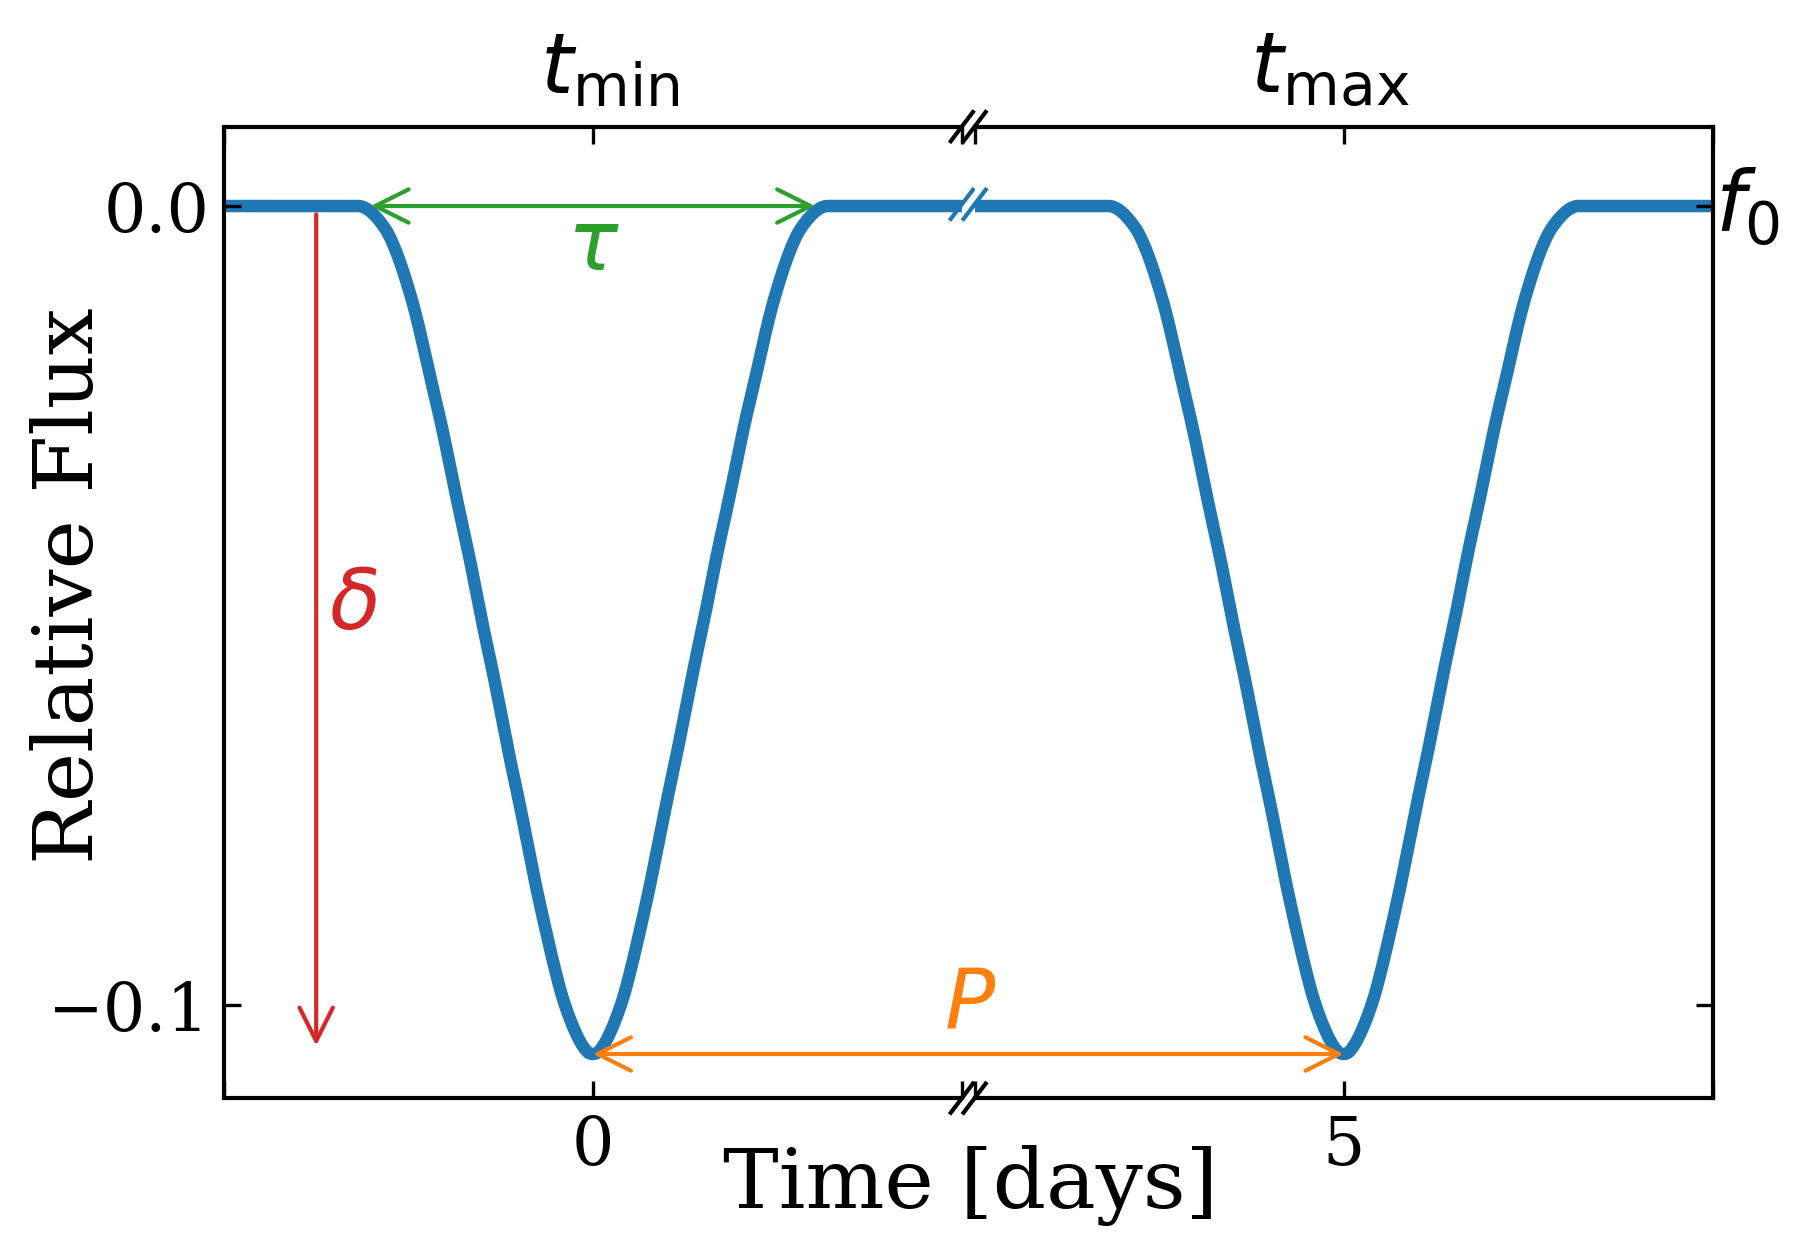
\includegraphics[width=\linewidth]{figures/transit_model.png}
  \caption{\textit{Schematic diagram of a transit light curve:} \alltodo{write some details about this plot}}
  \label{fig:schematic-transit-plot}
\end{figure}

More discussion of the details, motivations, and limitations of this transit parameterisation are presented below.

\paragraph{Transit times}
To speed up the analysis, we assume that the discovery period and phase of the orbit are close enough to the truth that we can fit only the data near the expected transit times.
One consequence of this assumption is that we are assuming that the \emph{number} of periods that occur in the \tess\ observational baseline is correct.
Practically, this means that our prior assumption is that the transits must occur within the data cutouts.
This can be difficult to enforce---especially for low signal-to-noise transits---but a good approximation can be achieved by fitting for two reference transit times, $t_{\rm min}$ and $t_{\rm max}$, with a fixed number of periods, $N_P$, between them, instead of a single reference time and the period.
Then we can compute the implied period as $P = (t_{\rm max} - t_{\rm min}) / N_P$.
Importantly this does not change the prior on $P$ and $t_0$ since the Jacobian is a constant $1/N_P$.

\paragraph{Transit depth}
It is worth spending a moment on the transit depth parameterisation.
This choice of parameterisation leads to efficient computation and convergence, but it comes with non-trivial shortcomings.
Since the physical parameter that is required to compute the light curve model is the radius ratio between the planet and the star $k = R_{\rm p} / R_\star$, we need to choose a parameterisation that is invertible and that isn't generally possible.
In some cases, using radius ratio directly as the parameter can work well, but \alltodo{explain cases where it's not}.
Instead, we choose to parameterise the approximate transit depth $\delta$ using the small planet approximation.
This is useful because it is directly invertible (conditioned on the limb darkening parameters and impact parameter), but it restricts us to considering non-grazing transits with impact parameter $|b| \le 1$.
Accepting this restriction, we can compute the approximate transit depth for a limb darkened light curve by assuming that the intensity of the star is uniform under the disk of the planet.
For quadratic limb darkening, the intensity profile is
\begin{equation}
  I(r) = 1 - u_1\,[1 - \mu(r)] - u_2\,[1 - \mu(r)]^2
\end{equation}
where $\mu(r) = \sqrt{1 - r^2}$.
The ratio of the occulted flux to the total stellar flux when the transit is deepest ($r = b$) is \citep[the same results are discussed by][]{Mandel:2002,Csizmadia:2013}
\begin{eqnarray}
  \delta &\approx& \frac{\int_0^k\,2\,\pi\,r\,I(b)\dd r}{\int_0^1\,2\,\pi\,r\,I(r)\dd r} \nonumber\\
  &=& \frac{k^2\,\left(1 - u_1\,[1 - \mu(b)] - u_2\,[1 - \mu(b)]^2\right)}{1 - u_1/3 - u_2/6}\quad.
\end{eqnarray}
Therefore, since $k$ must be positive, we have a one-to-one transformation between $\delta$ and $k$ conditioned on impact parameter $|b| \le 1$ and the limb darkening coefficients.
It is also important to include the Jacobian factor so that fitting in $\delta$ doesn't introduce a strange prior on $r$.
In this case, the relevant factor is
\begin{equation}
  \left|\frac{\dd k}{\dd \delta}\right| = \left|\frac{1 - u_1/3 - u_2/6}{2\,k\,\left(1 - u_1\,[1 - \mu(b)] - u_2\,[1 - \mu(b)]^2\right)}\right| \quad.
\end{equation}

\paragraph{Impact parameter}
Constrained to be non-grazing. -- \alltodo{Discuss the consequences of this.}

\paragraph{Transit duration}
The physical parameter required for computing the transit model is the semi-major axis, $a$, in units of the stellar radius, but the transit duration $\tau$ is better constrained so it can be better as a fit parameter.
For a circular orbit, the transit duration is \citep{Winn:2010}
\begin{equation}
  \tau = \frac{P}{\pi}\,\sin^{-1}\left( \frac{\sqrt{(1 + k^2) - b^2}}{a\,\sin i} \right) \quad.
\end{equation}
Rearranging this, we find
\begin{equation}
  a^2\,\sin^2 i\,\sin^2\left(\frac{\pi\,\tau}{P}\right) = (1 + k^2) - b^2 \quad.
\end{equation}
Then, using the fact that $\cos^2 i = b^2 / a^2$, we find
\begin{equation}
  a^2 = \frac{(1 + k)^2 - b^2\,\cos^2\phi}{\sin^2\phi}
\end{equation}
for $\phi = \pi\,\tau / P$.
And the Jacobian is
\begin{eqnarray}
  \frac{\dd a}{\dd \tau} &=& \frac{\pi\,\cos \phi}{a\,P\,\sin^3 \phi}\,\left[b^2 - (1 + k)^2\right] \quad.
\end{eqnarray}

Finally, from the period and semi-major axis, we can compute the implied stellar density (under this assumption of a circular orbit)
\begin{equation}
  \rho_\mathrm{circ} = \frac{3\,\pi\,a^3}{G\,P^2} \quad.
\end{equation}
It is important to note that this is not necessarily the same as the actual stellar density and that, in a multi-planet system, this implied density won't be the same for each planet \citep[see, for example,][]{Dawson:2012, Kipping:2012}.




\subsection{Bayesian Framework}


Likelihood, GP, Priors, \celerite, pymc3 sampling

%
%
%GPs are stochastic models consisting of a mean function
%$\mu_\vec{\theta}(\vec{x})$ and a covariance, autocorrelation, or ``kernel''
%function $K$ parameterized by
%$\vec{\theta}$ and $\vec{\alpha}$ respectively.
%Under this model, the log-likelihood function $\mathcal{L}
%(\vec{\theta},\,\vec{\alpha})$ with a dataset
%
%\begin{align}\eqlabel{gp-likelihood}
%\ln \mathcal{L} (\vec{\theta},\,\vec{\alpha})
%&= -\frac{1}{2} r(\vec{\theta})^{T}\, K(\vec{\alpha})^{-1}\, r(\vec{\theta}) \nonumber \\
%   -\frac{1}{2} \log \det K(\vec{\alpha})
%
%\end{align}






\section{Results}\label{sec:results}

\subsection{Systems with multiple planets}
Some words about these systems

\subsection{Planets with data for one transit}
Some stuff about single transit systems 


\section{Data and software availability}\label{sec:data}
We provide software to reproduce the analyses and results at \atlasUrl. 
The website contains one Jupyter notebook for each TOI, demonstrating the end-to-end analysis of a TOI. 
The notebooks contain software to download and clean light curve data, implementations of the transit-model and priors for inference, the \pymc sampling stage, and a posterior post-processing step.
The website also documents the method to download our Bayesian parameter inference posterior samples, load them and make various plots.  

\section{Discussion}\label{sec:conclusion}
We present for the first time a catalog of Bayesian posterior samples for the 2-minute cadence TOIs from 2018-2022. 
Some words about results. 
Some stuff about difficulty sampling grazing systems.
Errors when SPOC estimates are off. 
We expect the remainder of the \tess\ extended mission will complete by September 2023, at which point an updated catalog will be produced.

\begin{acknowledgments}

We would like to thank xyz. 
Ozgrav, Flatiron, NECTAR, ADACS, David Liptai
Work was started during `online.tess.science`

This work has made use of the TIC through the TESS Science Office’s target selection working group (architects K. Stassun, J. Pepper, N. De Lee, M. Paegert, R. Oelkers).

This research has made use of the NASA Exoplanet Archive, which is operated by the California Institute of Technology, under contract with the National Aeronautics and Space Administration under the Exoplanet Exploration Program.

This work made use of the \tess\ catalog on ExoFOP

Total compute time for this work \red{\cpuHrs} \alltodo{get more accurate compute time (this is an overestimate)}. CO$_2$ emission amount for this work would be XX, however as OzStar uses wind energy this has a negligible carbon footprint. 

\end{acknowledgments}

\vspace{5mm}
\facilities{\tess, \gaia, \kepler, Exoplanet Archive, etc.}

\software{
astropy \citep{Astropy-Collaboration:2013,Astropy-Collaboration:2018},  
exoplanet,
lightkurve, 
starry, 
celerite2,
pymc3,
numpy, 
scipy, 
pandas, 
matplotlib,
corner, 
sphinx, 
}


\bibliography{atlas}{}
\bibliographystyle{aasjournal}

\end{document}
